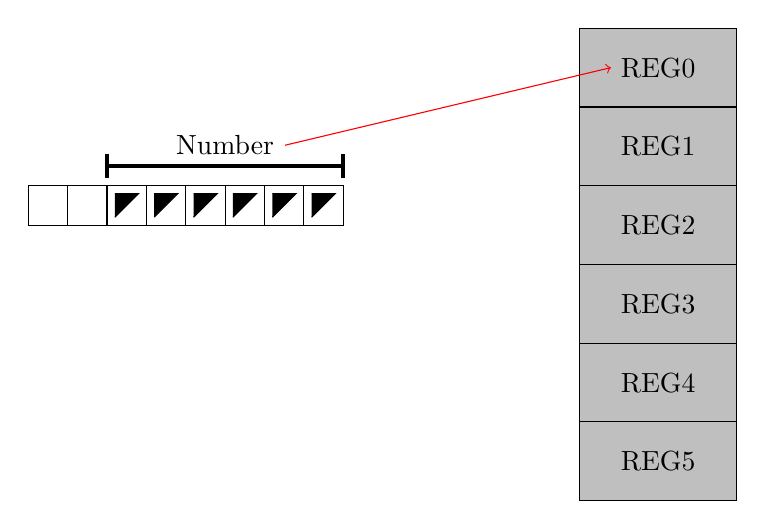
\begin{tikzpicture}
    \filldraw[fill=lightgray] (0,0) rectangle (2,1) node[pos=.5] {REG5};
    \filldraw[fill=lightgray] (0,1) rectangle (2,2) node[pos=.5] {REG4};
    \filldraw[fill=lightgray] (0,2) rectangle (2,3) node[pos=.5] {REG3};
    \filldraw[fill=lightgray] (0,3) rectangle (2,4) node[pos=.5] {REG2};
    \filldraw[fill=lightgray] (0,4) rectangle (2,5) node[pos=.5] {REG1};
    \filldraw[fill=lightgray] (0,5) rectangle (2,6) node[pos=.5] (reg0) {REG0};

    \foreach \x in {-7,-6.5,...,-6}{
        \draw (\x,4) rectangle (\x+0.5,3.5);
    }
        
    \foreach \x in {-6,-5.5,...,-3.5}{
        \draw (\x,4) rectangle (\x+0.5,3.5);
        \filldraw[fill=black] (\x+0.1,3.9) -- (\x+0.4,3.9) -- (\x+0.1,3.6);
    }

    \draw [line width=0.5mm](-6,4.4) -- (-6,4.1);
    \draw [line width=0.5mm](-3,4.4) -- (-3,4.1);
    \draw [line width=0.5mm](-6,4.25) -- (-3,4.25) node[pos=.5, above] (N) {Number};

    \draw [->,red] (N.east) to (reg0.west);
\end{tikzpicture}